\documentclass[a4paper,10pt,twocolumn]{article}
\usepackage{amsmath,booktabs,tabularx,array,graphicx,geometry,caption,xcolor,hyperref,xurl,microtype,longtable,pdflscape}
\usepackage[authoryear,round,sort]{natbib}
\setcitestyle{authoryear,open={(},close={)},citesep={;},aysep={}}
\geometry{top=2cm,bottom=2cm,left=2cm,right=2cm}
\graphicspath{{figures/}}
\setlength{\columnsep}{0.65cm}
\setlength{\parindent}{1.2em}
\setlength{\parskip}{0pt}
\setlength{\tabcolsep}{3pt}
\let\defaultthebibliography\thebibliography
\renewcommand{\thebibliography}[1]{%
  \defaultthebibliography{#1}%
  \setlength{\itemsep}{0pt}%
  \setlength{\parsep}{0pt}%
  \linespread{0.96}\selectfont%
}
\renewcommand{\arraystretch}{1.05}
\newcolumntype{Y}{>{\raggedright\arraybackslash}X}
\newcolumntype{L}[1]{>{\raggedright\arraybackslash}p{#1}}
\captionsetup{font=small,labelfont=bf,labelsep=period}
\setcounter{topnumber}{3}
\setcounter{bottomnumber}{2}
\setcounter{totalnumber}{5}
\renewcommand{\topfraction}{0.90}
\renewcommand{\bottomfraction}{0.75}
\renewcommand{\textfraction}{0.08}
\renewcommand{\floatpagefraction}{0.82}
\hypersetup{colorlinks=true,linkcolor=blue,citecolor=blue,urlcolor=blue,pdftitle={Multi-Sensor NDVI-Based FVC Retrieval Agreement with Copernicus FCOVER on a Common 300 m Target Grid: Geographic Heterogeneity and Historical-Window Transfer across Qinghai Plateau AOIs}}
\urlstyle{same}
\providecommand{\doi}[1]{\href{https://doi.org/#1}{https://doi.org/#1}}
\title{%
  {\fontsize{17}{19}\selectfont\bfseries
  Multi-Sensor NDVI-Based FVC Retrieval Agreement\\
  with \mbox{Copernicus FCOVER} on a Common \mbox{300 m} Target Grid:\par}
  \vspace{0.55em}
  {\fontsize{13}{15}\selectfont\normalfont
  Geographic Heterogeneity and Historical-Window Transfer\\
  across \mbox{Qinghai Plateau AOIs}\par}
}
\author{Hank Chen\thanks{Corresponding author: \href{mailto:13269982528@163.com}{13269982528@163.com}}}
\date{}
\begin{document}
\emergencystretch=1.5em
\pagestyle{plain}
\maketitle
\begin{abstract}
Direct native-resolution comparison with 300 m FCOVER can confound retrieval disagreement with target-grid mismatch. We harmonized Sentinel-2, Landsat 8/9, and MODIS NDVI to the native FCOVER grid, replicated the protocol across four deliberately selected contrasting Qinghai Plateau areas of interest (AOIs), and combined block-grouped diagnostics with chronological historical-window evaluation. The 2021--2025 design comprised 144 formal OLS runs and 48 target-year NDVI-based dimidiate pixel model (DPM) configurations. Mean 2025 Multi-AOI OLS RMSE was 0.041023 for Sentinel-2, 0.036840 for Landsat, and 0.030787 for MODIS (unweighted means of 24 runs per sensor). Agreement, preferred histories, and coefficients varied strongly by AOI; these summaries do not provide cross-sensor inferential rankings. Selected OLS errors were lower than selected DPM errors in all 12 sensor--AOI comparisons, but this secondary benchmark used empirical target-year NDVI endpoints and retrospectively selected minima. All 72 Rolling-Origin runs completed; trajectories and paired 5 km block contrasts showed no uniform association between longer historical-window configurations and lower forward error. Primary geographic and historical-transfer interpretations were qualitatively robust to aggregation-order, non-overlapping temporal-composition, and Landsat aerosol-QA sensitivities. The common target grid removes a direct native-pixel-versus-FCOVER-grid comparison but not support differences after QA. Results quantify agreement with an operational FCOVER reference, not field-level FVC accuracy.
\end{abstract}
\noindent\textbf{Keywords:} fractional vegetation cover; NDVI; Copernicus FCOVER; common target grid; Rolling-Origin evaluation; spatial validation

\section{Introduction}
Fractional vegetation cover (FVC) supports ecosystem and land-degradation assessment in arid and alpine settings \citep{chen2016uav,li2019plateau,han2023}. NDVI \citep{tucker1979} is widely used in calibrated FVC mappings and in the dimidiate pixel model (DPM), a two-endmember formulation \citep{carlson1997,gutman1998,jiapaer2011,yan2022dpm}. DPM transparency is offset by sensitivity to background, endmembers, shadow, and departures from two-component mixing \citep{huete1988,montandon2008,mu2024}; calibrated multi-source retrievals instead require matched references and transfer assessment \citep{wang2018fvc,mu2021multisource,song2022fvc}.

Copernicus FCOVER V2 RT6 is a 300 m, 10-day operational green-cover product with documented retrieval and validation history \citep{baret2013,camacho2013,liu2019,fuster2020,copernicus2025validation,copernicus2026atbd,copernicus2026pum}. Sentinel-2, Landsat, and MODIS differ in support, spectral response, timing, geometry, and QA \citep{drusch2012,roy2014,vermote2016}; residual NDVI differences remain after product-level correction \citep{claverie2018,zhang2018ndvi,shang2019,trevisiol2024}. Because observation support affects remotely sensed values and variance \citep{woodcock1987,atkinson2000}, direct comparison of native pixels with 300 m FCOVER can mix retrieval disagreement with grid mismatch.

Existing work generally treats FVC/DPM formulation, FCOVER validation, sensor harmonization, and spatial or chronological validation separately \citep{roberts2017,meyer2018,ploton2020,tashman2000,bergmeir2012}. The present study integrates common-target-grid harmonization, geographic replication, block-grouped diagnostics, and chronological transfer to test whether a simple NDVI--FCOVER relation is stable across those dimensions.

We evaluate (RQ1) common-target-grid FCOVER-reference agreement and the empirical-quantile DPM comparator across four AOIs; (RQ2) variation in error, history preference, and OLS coefficients; and (RQ3) whether longer histories are uniformly associated with lower 2024/2025 forward error. The design is an evaluation contribution, not a new retrieval algorithm: it neither identifies a causal effect of added years nor establishes field-level FVC accuracy.

\section{Methods}
\subsection{Study areas, products, and native preprocessing}
We evaluated four approximately 583 km$^2$ deliberately selected contrasting AOIs (Figure~\ref{fig:design}): AOI-00 ($99.51^{\circ}$E, $38.04^{\circ}$N), AOI-01 ($93.50^{\circ}$E, $36.50^{\circ}$N), AOI-02 ($95.60^{\circ}$E, $32.90^{\circ}$N), and AOI-03 ($97.20^{\circ}$E, $35.70^{\circ}$N). Selection used geographic separation, terrain, land-cover information, and 2021--2024 NDVI, not FCOVER numeric values or model performance. These deliberate contrasts are not a probability sample of the plateau.

Sentinel-2 Harmonized surface reflectance, Landsat 8/9 Collection 2 Level-2 Tier-1 surface reflectance, MOD09Q1 Collection 6.1, and Copernicus FCOVER V2 RT6 were analysed for 2021--2025 at 20 July, 31 July, and 10 August (Table~\ref{tab:data}) \citep{esa2015sentinel,s2harmonized,s2products,s2processing,usgslandsat,landsatscale,landsatqa,nasamodis,mod09c61}. Range screening and native QA preceded NDVI; rejected pixels were NoData, never zero-filled. Table~\ref{tab:data} gives the authoritative bands, scaling, and detailed flags. Sentinel-2 retained the specified SCL classes and finite cloud probability below 30\%; Landsat excluded the listed QA\_PIXEL and QA\_RADSAT conditions, with no additional aerosol-specific screen in the primary analysis. Landsat Collection 2 Level-2 surface reflectance is already atmospherically corrected. MODIS retained clear, quality-controlled land observations under its State and QC rules.

FCOVER was the native 300 m V2 RT6 grid (V2.0.1), not a resampled sensor product. Stored DN was scaled as $F=0.004DN$; pairing required non-NoData FCOVER, QFLAG, and NOBS, a true \texttt{valid\_domain\_mask}, QFLAG $<255$, NOBS $>0$, and $0\le F\le1$. QFLAG was not independently interpreted by quality class, and no FCOVER reference-quality sensitivity subset was evaluated.

\begin{table*}[!t]\centering\footnotesize
\caption{Products, native variables, scaling, and essential retained QA. Rejected source pixels were NoData, never zero-filled.}\label{tab:data}
\begin{tabularx}{.98\textwidth}{L{3.20cm}L{2.05cm}L{2.40cm}Y}\toprule
Product & Resolution; bands & Scaling & Essential retained QA logic \\\midrule
Sentinel-2 SR Harmonized & 10 m; B4/B8 & $\rho=10^{-4}\,DN$ & $1\le DN\le10{,}000$; SCL 4, 5, or 7; finite cloud probability $<30$\%. Harmonized export was used without an additional BOA offset. \\
Landsat 8/9 C2 L2 Tier 1 & 30 m; SR\_B4/\allowbreak SR\_B5 & $\rho=2.75\times10^{-5}DN-0.2$ & $7273\le DN\le43{,}636$; reject QA\_PIXEL bits 0--5 and 7 and any QA\_RADSAT flag. Primary analysis had no additional aerosol-specific screen; verified SR\_QA\_AEROSOL modes were assessed separately. \\
MOD09Q1 C6.1 & 250 m sinusoidal; b01/b02 & $\rho=10^{-4}DN$ & $-100\le DN\le16{,}000$; clear land, acceptable aerosol, no shadow/cirrus/snow/fire/cloud flags; MODLAND 0--1, band quality 0, atmospheric correction present. Valid negative reflectance was retained. \\
Copernicus FCOVER V2 RT6 & Native 300 m EPSG:\allowbreak 4326 grid & $F=0.004DN$ & Native NoData excluded; QFLAG $<255$, NOBS $>0$, derived valid-domain mask true, and $0\le F\le1$. \\\bottomrule
\end{tabularx}
\end{table*}


\subsection{NDVI, common target grid, and temporal composites}
For every QA-retained native pixel, NDVI was calculated as
\begin{equation}
\mathrm{NDVI}=\frac{\rho_{\mathrm{NIR}}-\rho_{\mathrm{red}}}{\rho_{\mathrm{NIR}}+\rho_{\mathrm{red}}},
\end{equation}
after finite scaled-band and nonzero-denominator checks. Source-grid NDVI was reduced directly to the native FCOVER grid with the mean reducer and FCOVER projection; FCOVER was not resampled, and no intermediate 10 m or 30 m raster was made. Thus native scaling and QA $\rightarrow$ native NDVI $\rightarrow$ aggregation $\rightarrow$ temporal compositing $\rightarrow$ FCOVER pairing defined the primary route. Mean native NDVI is not equivalent to NDVI from aggregated reflectance; this distinction was evaluated in the additional sensitivity analyses below.

The common 300 m target grid does not imply identical effective valid support. No per-cell valid-area fraction, overlap denominator, minimum native-pixel count, AOI-edge fraction, or additional coverage threshold was imposed; a cell was retained when its aggregated NDVI was finite. For each nominal date, the inclusive $\pm15$ d cell-wise median required at least two finite 300 m NDVI contributions. These nominal-date windows overlap and are not independent temporal replicates. MOD09Q1 is already an 8-day best-observation product, so this median is a second compositing stage. Cross-sensor target identities can differ after QA.

\begin{figure*}[!t]
\centering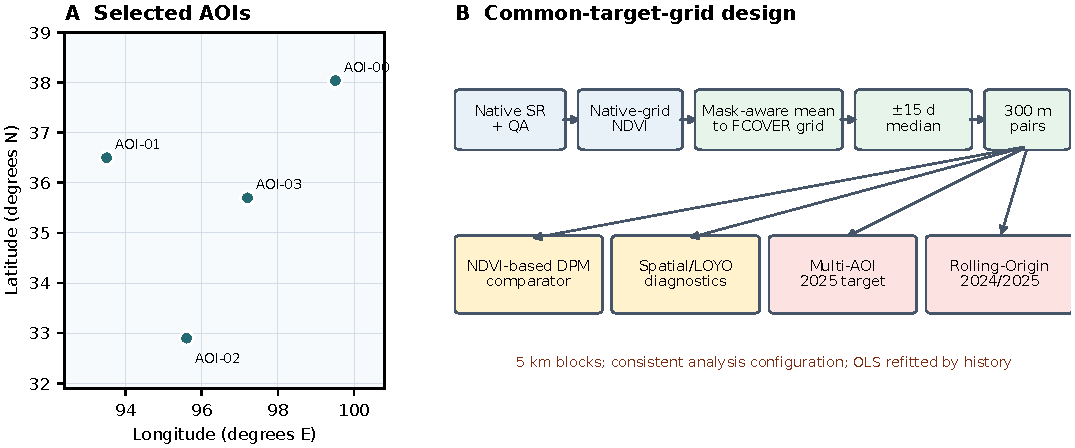
\includegraphics[width=.99\textwidth]{fig01_combined.pdf}
\caption{(A) Four deliberately selected contrasting Qinghai Plateau AOIs. (B) Native QA and NDVI preceded aggregation to the native FCOVER grid; spatial, geographic, and chronological evaluations supplied complementary evidence.}
\label{fig:design}
\end{figure*}

\subsection{Historical windows, blocks, and validation axes}
The 2025 Multi-AOI matrix crossed three sensors, four AOIs, and six histories (2022, 2023, 2024, 2022--2023, 2023--2024, and 2022--2024), yielding 72 independently fitted runs. Rolling-Origin evaluation used H1--H3 = 2023, 2022--2023, and 2021--2023 for target 2024, and 2024, 2023--2024, and 2022--2024 for target 2025. Three sensors $\times$ four AOIs $\times$ two targets $\times$ three depths yielded another 72 runs, for 144 formal OLS runs. The study separately executed 48 DPM benchmark configurations (four AOIs $\times$ three sensors $\times$ four endmember pairs). Target or later-year FCOVER never entered an OLS fit.

For every multi-year fit, a block was retained only if it contained valid pairs in every constituent year; eligible pairs were pooled in intercept-inclusive OLS. Years are consequently weighted by available pairs, not explicitly equally. A window can change constituent years, blocks, pair counts, and implicit weights, so the design does not isolate a causal effect of adding years. The 2025 H1/H2/H3 fits use the same complete-block rule as their nominally corresponding Multi-AOI histories.

FCOVER-cell centers were transformed to EPSG:32647 and assigned an AOI-namespaced block identifier using a fixed 5 km grid:
\begin{equation}
c=\left\lfloor\frac{x-525000}{5000}\right\rfloor,\qquad
r=\left\lfloor\frac{y-4195000}{5000}\right\rfloor.
\end{equation}
The block rule was stable across years. EPSG:32647 is used uniformly, although AOI-01 lies west of the conventional UTM zone; its point-scale factor at the AOI centre is 1.00259 (versus 0.99962--1.00085 for the other AOI centres). Thus ``5 km'' is an approximate grouping scale, not a claim of equal ground distance everywhere.

For diagnostics, blocks were deterministically ranked by SHA-256 of \texttt{42-block\_id}; the first rounded 20\% formed a reserve. Development blocks supplied five-fold GroupKFold and LOYO for multi-year histories. GroupKFold is a block-grouped within-domain diagnostic, not buffered spatial extrapolation; LOYO holds out one constituent year and is inapplicable to single-year histories. The reserve was evaluated before refitting, not used for tuning, selection, or inference, and recombined before the prescribed full fit; it is therefore not an independent final test. These axes complement the Multi-AOI target, Rolling-Origin target, DPM comparator, and block inference.

\subsection{Retrieval models, metrics, and inference}
For each sensor, AOI, and historical window, we fit an intercept-inclusive OLS relation on paired NDVI--FCOVER values and clipped only its predictions:
\begin{equation}
\widehat{\mathrm{FVC}}_{\mathrm{OLS}}=\operatorname{clip}(a\,\mathrm{NDVI}+b,0,1).
\end{equation}
Clipping was not part of coefficient estimation. The secondary benchmark was an NDVI-based DPM,
\begin{equation}
\widehat{\mathrm{FVC}}_{\mathrm{DPM}}=\operatorname{clip}\!\left(\frac{\mathrm{NDVI}-\mathrm{NDVI}_{\rm low}}{\mathrm{NDVI}_{\rm high}-\mathrm{NDVI}_{\rm low}},0,1\right),
\end{equation}
For each AOI $\times$ sensor, finite 2025 NDVI values from eligible paired identities across dates defined prespecified P1/P99, P2/P98, P5/P95, and P10/P90 endpoint pairs. No target-year FCOVER numeric value entered endpoint estimation. Endpoints are empirical proxies, not measured pure endmembers. Predictions were clipped to $[0,1]$ and evaluated on the corresponding valid target identities. The displayed DPM and OLS minima were both retrospectively selected by 2025 RMSE; their comparison is secondary and descriptive under unequal information conditions \citep{gutman1998,huete1988,montandon2008,jiapaer2011,yan2022dpm,mu2024}.

Endpoint sensitivity was quantified across all four prespecified DPM pairs for every sensor--AOI target sample as the range of RMSE, Bias, endpoint spread, and clipping fraction. Raw predictions were retained before clipping so that RMSE, MAE, and Bias could be compared before and after the fixed $[0,1]$ constraint. AOI-01 additionally received zero and historical-training-mean constant baselines using the exact complete-block historical sample of each OLS fit; target-year FCOVER was used only to evaluate those predictions. Thus neither DPM endpoints nor the predictive baselines use target-year FCOVER for construction. The primary OLS and DPM definitions, their target identities, and the existing retrospective selection rule were otherwise unchanged.

For $n$ valid target pairs, with $e_i=\widehat F_i-F_i$, we report
\begin{equation}
\begin{aligned}
\mathrm{RMSE}&=\sqrt{\frac{1}{n}\sum_{i=1}^{n}e_i^2},\qquad
\mathrm{MAE}=\frac{1}{n}\sum_{i=1}^{n}|e_i|,\\
\mathrm{Bias}&=\frac{1}{n}\sum_{i=1}^{n}e_i.
\end{aligned}
\end{equation}
Bias is prediction minus FCOVER. We also report $R^2$ and Pearson $r$; $r$ was undefined when either vector had zero variance \citep{willmott2005,chai2014}.

Rolling-Origin inference used paired 5 km block RMSE, not individual pixels, as its inferential unit. For each sensor--AOI--target-year contrast, every history was applied to the same eligible target-year AOI $\times$ nominal-date $\times$ FCOVER-grid-cell identities; the two block RMSE values were then joined by block identifier. Thus the paired block contrast compares predictions over identical target identities within each paired block, although the histories can have different training blocks and pair counts. For each contrast, $n$ was the number of blocks available in both compared histories, and $d_b=\mathrm{RMSE}_{\rm left,b}-\mathrm{RMSE}_{\rm right,b}$ was evaluated with a two-sided paired $t$ test: $\bar d$, its sample SD, $SE=s_d/\sqrt n$, $t=\bar d/SE$, and $df=n-1$. The reported 95\% confidence interval is $\bar d\pm t_{0.975,df}SE$. The 24 predefined sensor $\times$ AOI $\times$ target-year families each contained the H1--H2, H1--H3, and H2--H3 contrasts. Holm correction at $\alpha=0.05$ was applied only within these three-contrast families \citep{holm1979}; no global correction was made over 72 contrasts. With $\Delta\mathrm{RMSE}=\mathrm{RMSE}_{\rm left}-\mathrm{RMSE}_{\rm right}$, a positive value means lower block RMSE for the longer right-hand configuration, whereas a negative value means higher block RMSE for that configuration. The manuscript-wide count is descriptive across separately corrected families. Block differences may retain spatial dependence; no block-size sensitivity, buffered spatial CV, spatial-autocorrelation, permutation, or bootstrap robustness analysis was executed.

\subsection{Additional sensitivity analyses}
Three production sensitivities perturbed one preprocessing decision while retaining the FCOVER pairing, historical-window definitions, OLS fitting, Rolling-Origin evaluation, metrics, and block-level inference. First, the primary native-QA $\rightarrow$ native-NDVI $\rightarrow$ mean-NDVI route was compared with matched native RED/NIR valid-pixel support, mean RED and mean NIR on the FCOVER grid, and NDVI calculated from those aggregates. The matched support isolates aggregation order as far as the available products allow. Second, the primary inclusive $\pm15$ d nominal-date composites were retained as overlapping windows; a sensitivity assigned each source observation within their original temporal support to at most one nearest nominal date before compositing (ties to the earlier date), eliminating nominal-date reuse without redefining the primary experiment. Third, Landsat aerosol sensitivity applied verified \texttt{SR\_QA\_AEROSOL} modes in addition to the existing Collection 2 Level-2 surface-reflectance processing: exclusion of high aerosol, valid non-interpolated retrievals without high aerosol, and a strict valid-retrieval climatology/low-aerosol subset. Operational and matched-identity comparisons are distinguished where the perturbation changes support.

\section{Results}
\subsection{Common-target-grid FCOVER-reference agreement}
The common-target-grid data contained 995,060 sensor-specific pairs: 367,236 Sentinel-2, 267,762 Landsat, and 360,062 MODIS. They represented 386,649 unique AOI--year--date--FCOVER-cell identities. All 60 AOI--sensor--year groups were usable; AOI-02 Landsat lacked 10 August 2021 and was not imputed. FCOVER support varied after native QA. AOI-01 was near zero in 2025 (mean 0.0003; SD 0.0017).

All 72 Multi-AOI runs completed. Mean RMSE was 0.041023 for Sentinel-2, 0.036840 for Landsat, and 0.030787 for MODIS (Table~\ref{tab:multiaoi}); each is an unweighted mean of 24 run-level values. AOI mean RMSE ranged from 0.00139 to 0.05674, exceeding differences among the sensor means. AOI-01 had small absolute errors but best-window $R^2$ of 0.357--0.423, consistent with range restriction.

\begin{table}[!t]\centering\footnotesize
\caption{Descriptive 2025 Multi-AOI performance across 24 runs per sensor. Each entry is the unweighted arithmetic mean of the 24 run-level values for that sensor. Cross-sensor inference was not performed.}\label{tab:multiaoi}
\begin{tabular}{lrrrrr}\toprule
Sensor & RMSE & MAE & Bias & $R^2$ & $r$ \\\midrule
Sentinel-2 & 0.04102 & 0.03134 & -0.00700 & 0.675 & 0.878 \\
Landsat & 0.03684 & 0.02862 & +0.00309 & 0.703 & 0.848 \\
MODIS & 0.03079 & 0.02403 & +0.00572 & 0.742 & 0.880 \\
\bottomrule\end{tabular}
\end{table}


\subsection{DPM benchmark}
All 48 DPM configurations completed. The selected endpoint pair was P1/P99 in 9/12 sensor--AOI comparisons, P2/P98 in 2/12, and P5/P95 in 1/12 (Table~\ref{tab:formulaols}). Selected OLS RMSE was lower in all 12 comparisons. Both displayed minima were retrospectively selected as defined in Methods. DPM/OLS RMSE ratios ranged from 3.07 to 358.47; the extreme ratio is associated with near-zero AOI-01 and a very small OLS denominator, and is not a universal algorithm ranking.

\begin{table*}[!t]\centering\scriptsize
\caption{2025 FCOVER-reference error for the selected DPM endmember pair and OLS history within each sensor--AOI target sample. $\Delta$RMSE is DPM minus OLS; selection and information conditions are defined in Methods.}\label{tab:formulaols}
\resizebox{\textwidth}{!}{%
\begin{tabular}{llrrrlrrrr}\toprule
Sensor & AOI & DPM pair & DPM RMSE & DPM MAE & OLS history & OLS RMSE & OLS MAE & $\Delta$RMSE & DPM/OLS \\\midrule
Sentinel-2 & AOI-00 & P2/P98 & 0.1936 & 0.1707 & 2022 & 0.0631 & 0.0512 & 0.1305 & 3.07 \\
 & AOI-01 & P1/P99 & 0.4215 & 0.3780 & 2022 & 0.0013 & 0.0004 & 0.4202 & 318.30 \\
 & AOI-02 & P1/P99 & 0.1800 & 0.1560 & 2022--2024 & 0.0584 & 0.0450 & 0.1216 & 3.08 \\
 & AOI-03 & P1/P99 & 0.2075 & 0.1720 & 2022 & 0.0395 & 0.0274 & 0.1680 & 5.25 \\\addlinespace
Landsat 8/9 & AOI-00 & P5/P95 & 0.2061 & 0.1807 & 2023 & 0.0476 & 0.0389 & 0.1585 & 4.33 \\
 & AOI-01 & P1/P99 & 0.4860 & 0.4497 & 2023 & 0.0014 & 0.0006 & 0.4846 & 358.47 \\
 & AOI-02 & P1/P99 & 0.2111 & 0.1911 & 2022 & 0.0564 & 0.0435 & 0.1547 & 3.74 \\
 & AOI-03 & P1/P99 & 0.2097 & 0.1740 & 2022 & 0.0353 & 0.0254 & 0.1744 & 5.95 \\\addlinespace
MODIS & AOI-00 & P2/P98 & 0.1948 & 0.1778 & 2022--2023 & 0.0389 & 0.0310 & 0.1559 & 5.01 \\
 & AOI-01 & P1/P99 & 0.4303 & 0.3816 & 2022 & 0.0014 & 0.0006 & 0.4289 & 307.92 \\
 & AOI-02 & P1/P99 & 0.2040 & 0.1863 & 2023 & 0.0482 & 0.0370 & 0.1558 & 4.24 \\
 & AOI-03 & P1/P99 & 0.2193 & 0.1900 & 2024 & 0.0283 & 0.0204 & 0.1911 & 7.75 \\\bottomrule
\end{tabular}%
}
\end{table*}


\subsection{DPM endpoint, baseline, and clipping sensitivity}
Across the 12 sensor--AOI groups, endpoint-driven DPM RMSE ranges were 0.0176--0.1715 (Supplementary Table S4). The selected endpoint was therefore not geographically invariant: the narrowest ranges occurred in AOI-02 (0.0176--0.0422), whereas AOI-03 had the largest ranges (0.1622--0.1715). AOI-01 was also endpoint-sensitive (0.0984--0.1471), but P1/P99 remained its best configuration for all three sensors. Its best DPM RMSE values were still 0.4215 (Sentinel-2), 0.4860 (Landsat 8/9), and 0.4303 (MODIS), with positive biases of 0.3780, 0.4497, and 0.3816. Thus changing empirical quantiles did not materially resolve AOI-01 overprediction; its restricted reference support remains consequential.

For the retrospectively displayed AOI-01 OLS histories, RMSE was 0.0013--0.0014 versus 0.0018 for the zero baseline and 0.0017--0.0018 for the training-mean baseline, yielding positive RMSE skill of 0.204--0.255 (Table~\ref{tab:aoi01-baseline-clipping}). The small absolute OLS error consequently contains modest predictive skill rather than being solely a zero-dominated artefact, although its magnitude remains range-dependent. Clipping affected 36.1--64.8\% of AOI-01 raw OLS predictions and reduced OLS RMSE by only 0.000059--0.000179. The best DPM configuration clipped about 2\% of predictions, but clipping reduced its RMSE by 0.0103--0.0652; endpoint choice and clipping therefore alter the reported DPM error without changing the AOI-01 conclusion.

\begin{table}[!t]\centering\scriptsize
\caption{AOI-01 baseline and clipping sensitivity for the retrospectively displayed OLS history. Baseline skill is $1-\mathrm{RMSE}_{OLS}/\mathrm{RMSE}_{baseline}$.}
\label{tab:aoi01-baseline-clipping}
\resizebox{\linewidth}{!}{%
\begin{tabular}{lrrrrrrrr}
\toprule
Sensor & OLS RMSE & Zero RMSE & Mean RMSE & Skill vs zero & Skill vs mean & OLS clip. & Best DPM RMSE & DPM clip. \\
\midrule
Sentinel-2 & 0.0013 & 0.0018 & 0.0018 & 0.255 & 0.245 & 0.647 & 0.4215 & 0.020 \\
Landsat 8/9 & 0.0014 & 0.0018 & 0.0017 & 0.226 & 0.212 & 0.377 & 0.4860 & 0.020 \\
MODIS & 0.0014 & 0.0018 & 0.0018 & 0.213 & 0.204 & 0.361 & 0.4303 & 0.020 \\
\bottomrule\end{tabular}%
}
\end{table}


\subsection{Geographic and historical dependence}
Preferred histories differed by sensor and AOI; no geographically invariant historical window emerged. Six-window slope ranges across the 12 sensor--AOI combinations were 0.0117--0.1182 and intercept ranges were 0.0004--0.0671 (Figure~\ref{fig:coefficients}). Within fixed histories, GroupKFold slope ranges had median 0.0374 and maximum 0.1049; intercept ranges had median 0.0060 and maximum 0.0461. These are fold dispersion, not confidence intervals. AOI-01 slopes (0.051--0.110) remain weakly identifiable because its reference distribution is narrow.

\begin{figure*}[!t]
\centering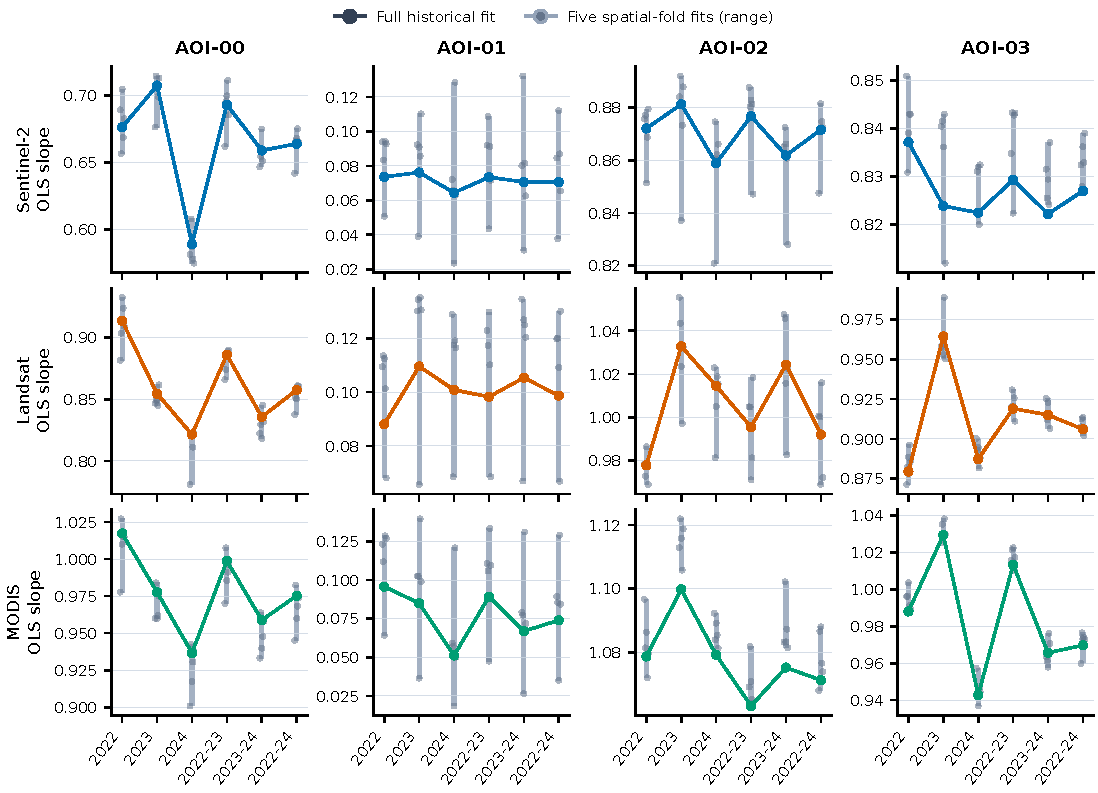
\includegraphics[width=.98\textwidth]{fig04_coefficient_stability.pdf}
\caption{Full-fit OLS slopes across six Multi-AOI histories. Grey points and segments show five existing GroupKFold fits and their ranges; they are descriptive spatial-fold dispersion, not confidence intervals. Vertical scales differ by panel.}
\label{fig:coefficients}
\end{figure*}

\subsection{Internal diagnostics and chronological transfer}
All applicable GroupKFold, LOYO, and historical-reserve diagnostics completed. Their broad variation by sensor and AOI produced no stable internal history ranking. The reserve was not used for tuning or inference and was recombined before the prescribed full fit; complete LOYO and reserve summaries are Supplementary Tables S2--S3.

All 72 Rolling-Origin runs completed. Figure~\ref{fig:rolling} shows no uniform monotonic relation between longer histories and lower forward error. Sensor-level mean RMSE for 2024/2025 was 0.03923/0.04099 for Sentinel-2, 0.03706/0.03716 for Landsat, and 0.03305/0.03091 for MODIS (unweighted means of 12 AOI--history runs per row).

\begin{figure*}[!t]
\centering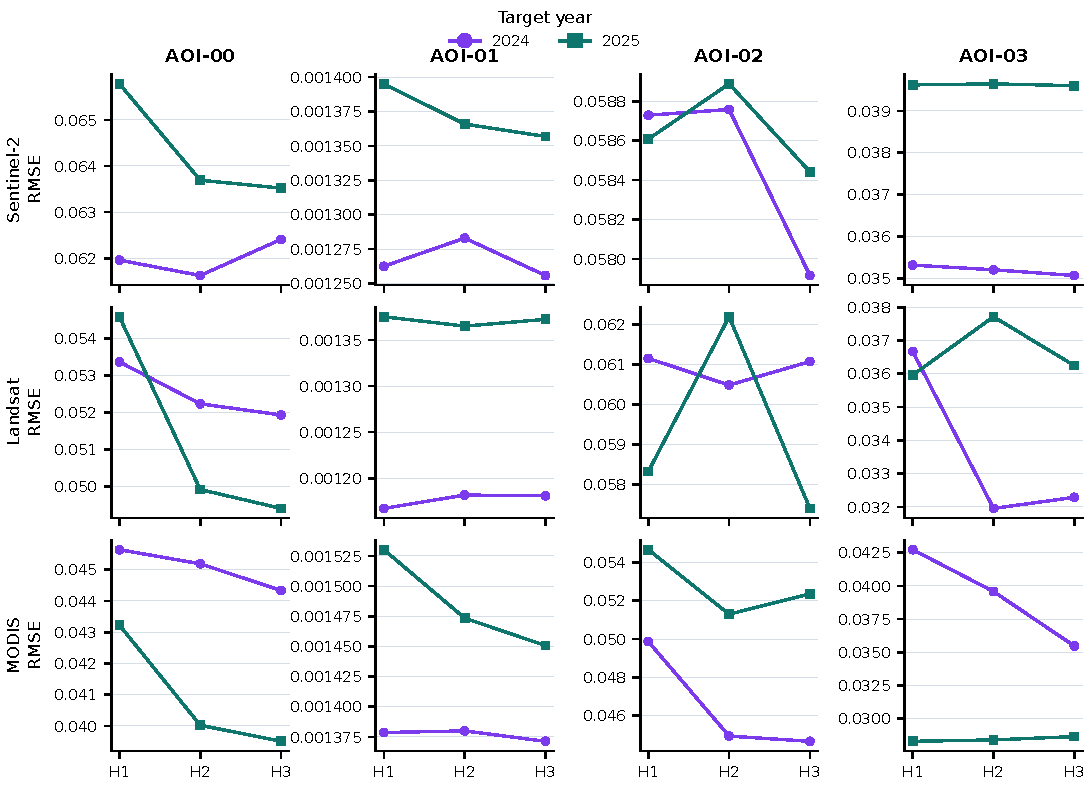
\includegraphics[width=.98\textwidth]{fig05_rolling_trajectories.pdf}
\caption{Rolling-Origin RMSE trajectories for one- to three-year histories (H1--H3); see Methods for the temporal-compositing design.}
\label{fig:rolling}
\end{figure*}

\subsection{Block-level contrasts}
Paired block contrasts were heterogeneous (Figure~\ref{fig:effects}; Table~\ref{tab:contrasts}). Of 72 predefined contrasts, 39 were Holm-supported within their corresponding local families: 30 favoured lower error and 9 higher error for the longer configuration. Eleven supported AOI-01 effects had $|\Delta\mathrm{RMSE}|<0.0001$. The largest supported lower-error contrast was MODIS AOI-03, 2024 H1--H3 ($\Delta\mathrm{RMSE}=+0.007654$); the largest supported higher-error contrast was Landsat AOI-02, 2025 H1--H2 ($-0.004124$). Complete statistics for all 72 contrasts are in Supplementary Table S1.

\begin{table*}[!t]\centering\footnotesize
\caption{Summary of paired block-RMSE contrasts on identical target identities. Positive left-minus-right differences mean lower error for the longer configuration; inferential procedures are defined in Methods.}\label{tab:contrasts}
\begin{tabular}{lrrrrr}\toprule
Sensor & Contrasts & Holm-supported & Longer-window lower error & Longer-window higher error & AOI-01 $|\Delta|<10^{-4}$ \\\midrule
Sentinel-2 & 24 & 6 & 4 & 2 & 4 \\
Landsat 8/9 & 24 & 17 & 13 & 4 & 4 \\
MODIS & 24 & 16 & 13 & 3 & 3 \\
All sensors & 72 & 39 & 30 & 9 & 11 \\
\bottomrule\end{tabular}
\end{table*}


\begin{figure*}[!t]
\centering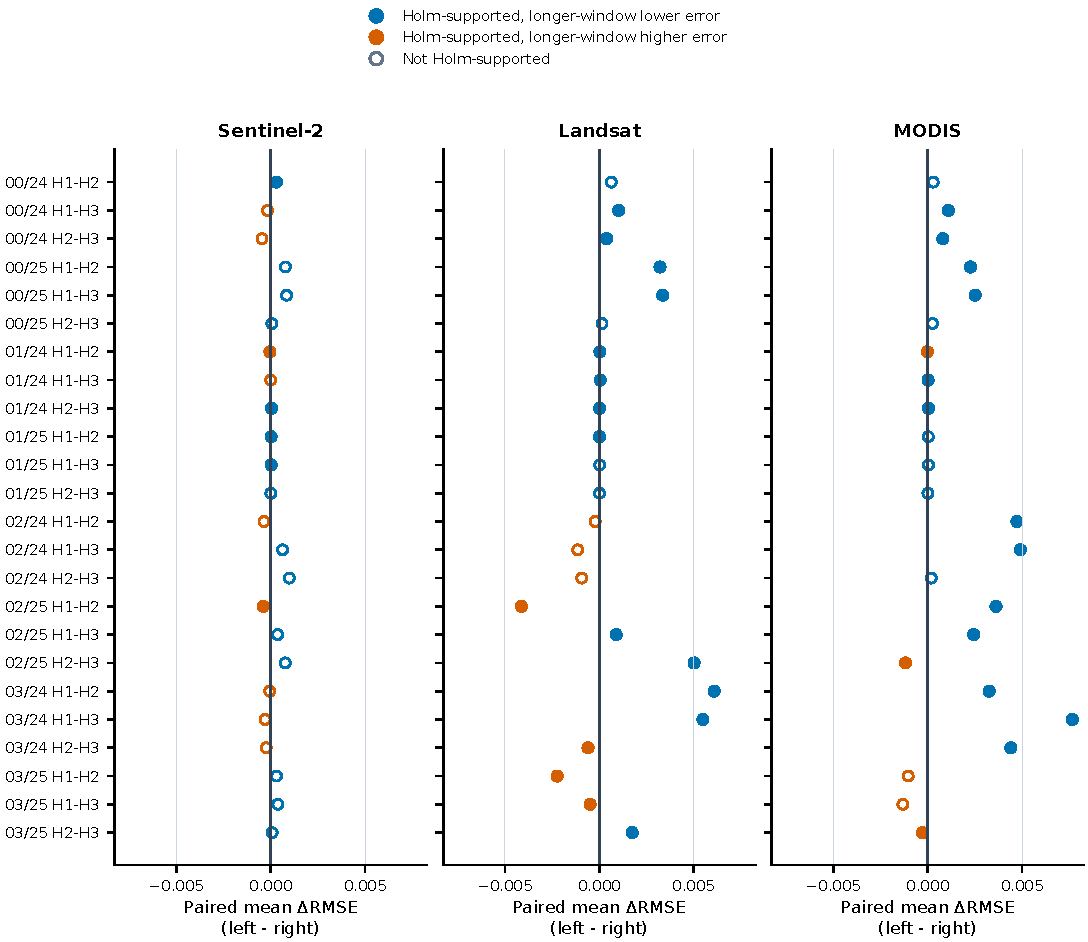
\includegraphics[width=.98\textwidth]{fig06_paired_effects.pdf}
\caption{All 72 paired block-RMSE contrasts. Positive left-minus-right values mean lower block RMSE for the longer configuration; negative values mean higher block RMSE. Filled markers denote within-family Holm support.}
\label{fig:effects}
\end{figure*}

\subsection{Additional sensitivity analyses}
The aggregation-order Route A reproduced the frozen primary outputs for all 13 checks, and the matched Route B comparison retained every target identity. Mean absolute matched $\Delta$NDVI ranged from 0.000101 to 0.006864; operational $\Delta$RMSE ranged from $-0.001458$ to $+0.000493$. One of 12 preferred histories changed (MODIS AOI-03), and two Rolling-Origin directions changed (both Sentinel-2). Thus the common-grid and geographic interpretations were robust to this ordering choice, although individual sensor--AOI estimates were quantitatively modified.

Under nearest-nominal non-overlap, source-assignment retention was 0.857--1.000 and duplicate source identities were zero; resulting target-pair retention was 0.132--0.992. Operational $\Delta$RMSE ranged from $-0.002319$ to $+0.014052$, whereas matched-identity $\Delta$RMSE ranged from $-0.000900$ to $+0.017763$. Seven of 12 preferred histories and three Rolling-Origin directions changed. These are respectively operational and matched-support comparisons, so their differences cannot all be attributed to overlap alone; nevertheless, removing nominal-date reuse did not produce a uniform longer-history advantage.

For Landsat, the valid modes were exclusion of high aerosol, valid-retrieval/no-high-aerosol, and strict valid-retrieval climatology/low-aerosol screening, each additional to the primary Level-2 surface-reflectance processing. Retention across AOI--year groups was 0.355--1.000. Operational and matched-identity $\Delta$RMSE ranges were $-0.003969$ to $+0.027036$ and $-0.001837$ to $+0.033996$, respectively; the largest increases occurred for strict screening in AOI-02 (2025 retention 0.396). Four of 12 preferred histories and nine Rolling-Origin directions changed. Additional aerosol-specific screening was therefore associated with substantial support loss and configuration-specific numerical changes, but did not alter the Landsat or cross-AOI manuscript conclusions (Table~\ref{tab:sensitivity}; Supplementary Table~S9).

\begin{table*}[!t]\centering\footnotesize
\caption{Robustness of primary conclusions under additional sensitivity analyses. Ranges are across the reported sensor--AOI configurations; $\Delta$RMSE is sensitivity minus primary. Operational and matched-identity comparisons are distinguished when support changes. Detailed results are in Supplementary Tables S7--S9 and the archived repository outputs.}\label{tab:sensitivity}
\begin{tabularx}{\textwidth}{L{2.35cm}L{1.55cm}Y Y Y Y}\toprule
Sensitivity & Scope & Support/sample effect & Performance effect & History/transfer effect & Interpretation \\\midrule
Aggregation order & 3 sensors, 4 AOIs & Matched target identities retained (1.000). Mean absolute matched $\Delta$NDVI: 0.000101--0.006864. & Operational $\Delta$RMSE: $-0.001458$ to $+0.000493$. & 1/12 preferred histories; 2/12 Rolling-Origin directions changed. & Geographic and common-grid conclusions robust; individual estimates quantitatively modified. \\
Non-overlapping temporal composition & 3 sensors, 4 AOIs & Source assignment: 0.857--1.000; resulting target pairs: 0.132--0.992; no duplicate source identities. & Operational $\Delta$RMSE: $-0.002319$ to $+0.014052$; matched: $-0.000900$ to $+0.017763$. & 7/12 preferred histories; 3/12 Rolling-Origin directions changed. & No uniform longer-history advantage after removing nominal-date reuse. \\
Landsat aerosol QA & 3 additional aerosol modes, 4 AOIs & AOI--year retention: 0.355--1.000; strict screening caused the greatest loss. & Operational $\Delta$RMSE: $-0.003969$ to $+0.027036$; matched: $-0.001837$ to $+0.033996$. & 4/12 preferred histories; 9/12 Rolling-Origin directions changed. & Landsat interpretation robust, with support-sensitive quantitative changes. \\
\bottomrule\end{tabularx}
\end{table*}


\section{Discussion}
\subsection{Common-grid agreement and geographic heterogeneity}
Harmonization to the FCOVER target grid removes a direct native-pixel-versus-300 m comparison, but not differences in spectral response, timing, atmosphere, geometry, QA, or effective valid support \citep{claverie2018,zhang2018ndvi,shang2019,trevisiol2024}. The matched aggregation-order sensitivity preserved all target identities and the geographic interpretation, although it modified some sensor--AOI estimates and one preferred history; it does not establish either aggregation order as universally correct. MODIS had the lowest mean RMSE in this protocol, but its native support and aggregation choice may contribute; this is not a universal sensor-capability ranking \citep{woodcock1987,atkinson2000}. Geographic variation exceeded the sensor-mean separation. AOI-01 particularly shows why low absolute error must be read with target range, $R^2$, and coefficient identifiability. The four AOIs reveal conditionality but are designed contrasts, not a regional probability sample \citep{roberts2017,meyer2018,ploton2020}.

\subsection{Historical-window transfer}
No history was geographically invariant, and Rolling-Origin results did not show monotonic benefit from longer windows. The primary $\pm15$ d windows overlap; the non-overlapping assignment changed several selected histories and directions, but preserved the absence of a uniform longer-history benefit. Coefficient drift and the diagnostic variation are consistent with changing NDVI--FCOVER relations across place and history. Because a historical window changes years, blocks, pair counts, and their implicit weights together, these results do not identify the effect of adding a year alone. The practical implication is to assess the intended domain with block-grouped diagnostics and chronological forward evaluation rather than treating record length as a universal tuning direction \citep{tashman2000,bergmeir2012}.

\subsection{DPM and practical implications}
The DPM results show that empirical-endpoint sensitivity is geographically conditional rather than invariant. AOI-02 was comparatively stable, while AOI-03 had the largest absolute endpoint-driven RMSE differences; AOI-01 was not uniquely unstable, although its P1/P99 empirical high-NDVI endpoint proxy still produced large positive bias. Narrowing the quantile range did not rescue AOI-01, indicating that its extreme DPM error reflects restricted FCOVER support and the empirical-reference-range mismatch in addition to endpoint parameterization. The AOI-01 OLS fits retained modest skill against zero and historical-mean baselines, but their low absolute errors should continue to be read with the restricted target range and the documented clipping frequency. DPM remains useful when paired calibration is unavailable, but empirical endpoints are not measured endmembers and estimates remain sensitive to background, shadow, and two-component assumptions \citep{huete1988,montandon2008,jiapaer2011,yan2022dpm,mu2024}. Configuration choice should therefore be evaluated in its intended geographic and temporal setting.

Landsat Collection 2 Level-2 surface reflectance was already atmospherically corrected in the primary analysis. Additional \texttt{SR\_QA\_AEROSOL} screening was associated with configuration-specific error changes, including large changes after strict filtering in AOI-02, rather than evidence that aerosol alone caused those differences. Its support loss under strict rules reinforces the need to report the retained sample and residual spectral, atmospheric, and support differences alongside any aerosol-screened result.

\section{Limitations}
Copernicus FCOVER is an operational product reference, not field ground truth; field, UAV, or validated high-resolution reference data would be required for absolute FVC accuracy \citep{baret2013,camacho2013,fuster2020,copernicus2025validation,mu2015sampling,chen2016uav,olofsson2014}. The four designed AOIs are not plateau probability samples. A common 300 m grid does not equalize effective valid support: no exact valid-area weighting, overlap denominator, or minimum native-pixel threshold was retained. Matched-support aggregation-order results bound one processing effect but do not resolve residual cross-sensor support differences or limitations of mean aggregation. Primary nominal-date windows overlap; the unique-assignment sensitivity removed duplicate source use but also changed support. Native QA cannot make acquisition, atmospheric, spectral, or support conditions equivalent across sensors, and valid target subsets can consequently differ. FCOVER validity followed the implemented QFLAG/NOBS rules, but QFLAG classes and FCOVER reference-quality subsets were not evaluated. Landsat aerosol screening was evaluated, but strict modes can materially reduce support and do not remove residual atmospheric or spectral differences.

Historical windows differ in years, blocks, pair counts, and implicit weights, so causal effects of historical depth cannot be isolated. Paired target identities were identical within a block contrast, but the corresponding training samples were not. The reserve was recombined before full fitting; GroupKFold was not buffered extrapolation; the AOI-01 block scale is approximate; and residual spatial dependence may remain. No block-size, autocorrelation, permutation, or bootstrap sensitivity was performed. DPM endpoints remain empirical proxies, and selected DPM/OLS minima were retrospectively selected from different candidate and information conditions. AOI-01's near-zero distribution still constrains interpretation, although clipping frequency and naïve-baseline performance are now quantified.

\section{Conclusion}
Common-target-grid harmonization enabled sensor-specific NDVI--FCOVER agreement assessment without direct native-pixel-versus-target-grid comparison. Across four AOIs, agreement, coefficients, and preferred histories were geographically conditional, and longer historical-window configurations were not uniformly associated with lower forward error. These interpretations were robust to the tested aggregation-order, non-overlapping-composition, and Landsat aerosol-QA sensitivities, despite configuration-specific numerical changes. The practical implication is to evaluate the intended-domain history with both block-grouped stability diagnostics and chronological forward testing, rather than select a configuration by record length alone. Reporting local contrast magnitude and direction alongside inference makes this decision transparent and guards against over-reading pooled summaries. Its role is to guide configuration evaluation, not to rank sensors. The common target grid reduces one source of mismatch but does not equalize valid support after QA. These findings concern agreement with Copernicus FCOVER and do not establish absolute field-level FVC accuracy.

\section*{Statements and Declarations}

\subsection*{Funding}
No funding was received for conducting this study.

\subsection*{Competing Interests}
The author declares no competing interests.

\subsection*{Author Contributions}
Hank Chen: Conceptualization, methodology, software, formal analysis, investigation, data curation, visualization, writing -- original draft, writing -- review and editing.

\subsection*{Ethics Approval}
Not applicable. This study analyzes remotely sensed satellite-product data and does not involve human participants, personal data, clinical research, animal subjects, or interventions.

\subsection*{Consent to Participate}
Not applicable.

\subsection*{Consent for Publication}
Not applicable.

\subsection*{Data Availability}
The source satellite products analyzed in this study are publicly accessible from their respective providers: Sentinel-2 Harmonized surface reflectance through Google Earth Engine; Landsat 8/9 Collection 2 Level-2 Tier-1 surface reflectance through the U.S. Geological Survey; MOD09Q1 Collection 6.1 through NASA/LP DAAC; and Copernicus FCOVER V2 RT6 through the Copernicus Land Monitoring Service \citep{s2harmonized,usgslandsat,mod09c61,copernicus2026pum}. The derived datasets supporting the analyses reported in this study, including paired NDVI--FCOVER data, run-level metrics, DPM and OLS results, block-level contrasts, LOYO outputs, historical-reserve outputs, source-scene manifests, and final tables, are openly available at \url{https://github.com/Han-chh/FVC-Report-repo}. No new field-observation dataset was collected for this study.

\subsection*{Code Availability}
The analysis code, archived analysis configurations, portable local reproduction runner, and tests used for this study are openly available at \url{https://github.com/Han-chh/FVC-Report-repo}.

\subsection*{Materials Availability}
Not applicable. No physical, biological, or experimental materials were used in this study.

\bibliographystyle{plainnat}
\bibliography{bibliography}
\end{document}
